% ======================================================
% Compile: xelatex 5state_aprime_mirror.tex
% Path:    reference/eq17_analysis/derivation/5state_aprime_mirror.tex
% The MIRROR (kappa~0) of the a'_hdm variance-ratio channel, told as three
% parallel tracks (True / Estimate / Error).  Companion (same notation/route):
%   5state_aprime_var_esti.tex   (esti-source self-reference, lumped kappa)
%   5state_aprime_var_chain.tex  (moving-trajectory leak, lambda_leak)
% This file isolates the HOLD mirror: why the online variance ratio reads back
% the controller's own a', not the truth, and why that kills the channel when
% fed back.  Verification figure (frozen-arm knife) at the end.
% ======================================================
% fontset=none: no CJK text; compiles anywhere.
\documentclass[11pt,a4paper,fontset=none]{ctexart}

\usepackage[fleqn]{amsmath}
\usepackage{amssymb,bm}
\usepackage{empheq}
\setlength{\mathindent}{0pt}
\usepackage{geometry}
\geometry{margin=2.0cm}
\usepackage{array,booktabs}
\usepackage{graphicx}

\setlength{\parindent}{0pt}
\setlength{\parskip}{0.3em}
\setlength{\abovedisplayskip}{4pt}
\setlength{\belowdisplayskip}{4pt}
\setlength{\abovedisplayshortskip}{2pt}
\setlength{\belowdisplayshortskip}{2pt}

\newcommand{\lc}{\lambda_c}
\newcommand{\ap}{{a'_{hd}}}
\newcommand{\aph}{{\hat a'_{hd}}}
\newcommand{\apm}{{a'_{hdm}}}
\newcommand{\apmh}{{\hat a'_{hdm}}}
\newcommand{\eap}{{e_{a'_h}}}
\newcommand{\hd}[1]{\par\medskip\noindent\underline{\textbf{#1}}\par\nobreak\vspace{0.2ex}}

\begin{document}

\begin{center}\large\textbf{The $\apm$ mirror ($\kappa\!\approx\!0$): three parallel tracks}\end{center}

The whole derivation answers one question: \emph{if the variance-ratio reading
$\apmh$ is fed to the $a'$ update, does the error $\eap=\ap-\aph$ shrink
(converge) or drift?}  The answer is built from three parallel tracks --
\textbf{True} (how $a_h,a',a_r$ really evolve), \textbf{Estimate} (how
$\aph,\hat a_r,\apmh$ are computed online), and \textbf{Error} $=$ True $-$
Estimate.  Section 3 is the bridge: it shows the Estimate track is a
\emph{mirror} of the controller's own $\aph$, not a measurement of $\ap$.

\hd{0. Definitions and $[k]$ timing}

\[
h[k] = h_d[k] - \delta h[k], \qquad
\Delta h_d[k] = h_d[k+1] - h_d[k]
\]
\[
\ap[k] := \left.\frac{d a_h}{d h}\right|_{h_d[k]}, \qquad
a_r[k] := a_h[k] - a_h\big(h_d[k]\big)
\]
\[
\delta h[k+1] = \lc\,\delta h[k] - F_{dh}[k]\,e_{a_h}[k] - \varepsilon_h[k]
\]
\[
a_{var} = a_{cov} = 0.05, \qquad
T_s = 1/1600, \qquad
\beta = 1 - T_s/\tau,\ \tau = 0.35\,\mathrm s \;\Rightarrow\; \beta = 0.99821
\]

\textbf{$[k]$ bookkeeping} (the telescoping in \S3 stands on this):
\[
\text{delay chain:}\quad \delta h_1[k]=\delta h[k-2],\ \ \delta h_2[k]=\delta h[k-1],\ \ \delta h_3[k]=\delta h[k]\ (\text{current, leading})
\]
\[
\text{measurement:}\quad y_1[k]=\delta x_m[k]=\delta h[k-d]+n_1\ \ \text{observes }\delta h_1,\ \ d=2;
\qquad y_2[k]=a_{xm}[k]\ \text{observes }\hat a_h
\]
\[
\text{per step:}\quad \underbrace{\text{predict}}_{\delta\hat h_3[j+1]=\lc\,\delta\hat h_3[j]}\ \longrightarrow\ \underbrace{\text{update}}_{\text{innovation }u}
\]

\hd{1. True (Track A)}

$a_h$ follows the real height. With
$h[k{+}1]-h[k]=\Delta h_d+(1-\lc)\delta h+F_{dh}e_{a_h}+\varepsilon_h$, a
first-order expansion (drop $a''$) gives
\[
a_h[k+1] \approx a_h[k] + \ap\,\Delta h_d + (1-\lc)\,\ap\,\delta h
+ \ap\,F_{dh}\,e_{a_h} + \ap\,\varepsilon_h
\]

\begin{empheq}[box=\fbox]{equation*}
\ap[k+1] \approx \ap[k], \qquad
a_r[k] = a_h[k]-a_h(h_d[k]) = -\,\ap[k]\,\delta h[k]
\end{empheq}

The anchor $a_r=-\ap\,\delta h$ is the whole channel's footing: taking variances,
\[
\apm[k] := +\sqrt{\;\mathrm{Var}(a_r[k]) \,/\, \mathrm{Var}(\delta h[k])\;}
= \ap[k] \qquad (\ap>0)
\]
In the True track the ratio recovers $\ap$ exactly. This is the gold standard the
online version is judged against (verified: fig., left panel, $a_r$ overlays
$-\ap\,\delta h$).

\hd{2. Estimate (Track B)}

Online there is no true $a_r,\delta h$ -- only the EKF estimates $\hat a_h,\delta\hat h_3$.
The same recipe is rebuilt from estimates with two EWMA stages each:
\[
\begin{aligned}
\overline a_h[k+1] &= (1-a_{var})\,\overline a_h[k] + a_{var}\,\hat a_h[k+1], &
\hat a_r[k] &= \hat a_h[k] - \overline a_h[k] \\
\hat\sigma^2_{\hat a_r}[k+1] &= (1-a_{cov})\,\hat\sigma^2_{\hat a_r}[k] + a_{cov}\,\hat a_r^2[k+1] & & \\[2pt]
\overline{\delta\hat h}[k+1] &= (1-a_{var})\,\overline{\delta\hat h}[k] + a_{var}\,\delta\hat h_3[k+1], &
\delta\hat h_r[k] &= \delta\hat h_3[k] - \overline{\delta\hat h}[k] \\
\hat\sigma^2_{\delta\hat h}[k+1] &= (1-a_{cov})\,\hat\sigma^2_{\delta\hat h}[k] + a_{cov}\,\delta\hat h_r^2[k+1] & &
\end{aligned}
\]

\begin{empheq}[box=\fbox]{equation*}
\apmh[k] := +\sqrt{\;\hat\sigma^2_{\hat a_r}[k] \,/\, \hat\sigma^2_{\delta\hat h}[k]\;}
\end{empheq}

This is the number that would feed the filter. The predict of $\hat a_h$ (\S4)
uses $\aph$ itself -- the seed of the mirror.

\hd{3. Telescoping $\to$ mirror (predict-only bridge)}

In a hold ($\Delta h_d=0$), predict-only ($u\equiv0$), the gain-state predict is
\[
\hat a_h[k+1] = \hat a_h[k] + (1-\lc)\,\aph\,\delta\hat h_3[k],
\qquad
(1-\lc)\,\delta\hat h_3[j] = \delta\hat h_3[j] - \delta\hat h_3[j+1]
\]
using $\delta\hat h_3[j+1]=\lc\,\delta\hat h_3[j]$ (\S0 predict). Summing from
$k_0$ telescopes the middle terms:
\[
\hat a_h[k] = \big[\hat a_h[k_0]+\aph\,\delta\hat h_3[k_0]\big] - \aph\,\delta\hat h_3[k]
= C - \aph\,\delta\hat h_3[k]
\]
The EWMA mean $\overline a_h$ removes the constant $C$, leaving

\begin{empheq}[box=\fbox]{equation*}
\hat a_r[k] = -\,\aph[k]\,\delta\hat h_r[k]
\qquad\Longrightarrow\qquad
\apmh[k] = \sqrt{\aph{}^2\,\hat\sigma^2_{\delta\hat h}/\hat\sigma^2_{\delta\hat h}} = \aph[k]
\quad \forall\,\aph
\end{empheq}

\textbf{Mirror}: the numerator $\hat\sigma^2_{\hat a_r}$ was built from $\hat a_h$,
which the controller integrated using its own $\aph$; so it reads $\aph{}^2$ (your
belief), not $\ap{}^2$ (truth). The shared $\delta\hat h$ cancels in the ratio and
returns your input. No truth enters.

\hd{4. $u\neq0$: the crack $\kappa$, and where $y_1$ contributes}

With the real filter ($u\neq0$) the innovation correction adds a term $u_r$ (truth
enters only through the $y_2$ innovation $\nu_2\approx-\eap\,\delta h_r[k-d]+n_2$):
\[
\hat a_r[k] = -\,\aph\,\delta\hat h_r[k] + u_r[k]
\]
\[
\mathrm E[\hat a_r^2]/\sigma^2_{\delta h}
= \aph{}^2 + \underbrace{2\aph\,\kappa\,\eap}_{\text{truth}} + \underbrace{\sigma^2_u/\sigma^2_{\delta h}}_{\text{floor}},
\qquad
\mathrm E[\delta\hat h_r\,u_r] =: -\kappa\,\eap\,\sigma^2_{\delta h}
\]
Linearising the square root, $\sqrt{\aph{}^2+\epsilon}\approx\aph+\epsilon/(2\aph)$,

\begin{empheq}[box=\fbox]{equation*}
\apmh[k] = \aph[k] + \kappa[k]\,\eap[k] + n_{var}[k],
\qquad
n_{var}=b_u+w,\quad b_u=\frac{\sigma^2_u}{2\,\aph\,\sigma^2_{\delta h}}
\end{empheq}

$\kappa$ is the crack through which truth enters ($\kappa=1$ measurement,
$\kappa=0$ pure mirror); $b_u>0$ is the sqrt-rectification floor, $\propto1/\aph$.

\textbf{Observability ($y_1$'s role)}: $y_1$ is not absent -- it \emph{shapes}
$\delta\hat h_r$, the signal shared by numerator and denominator, so it reinforces
the mirror rather than breaking it. But in a hold $y_1$ is \emph{blind} to $a'$:
$\eap$ reaches $\delta h$ only through $F_e(4,5)=\Delta h_d$ (\S6), which is gated
to $0$; hence $y_1$ contributes nothing to $\kappa$. All of $\kappa$ (tiny) comes
from $y_2$.

\hd{5. Error (Track C $=$ A $-$ B)}

Subtract the two $a'$ updates. Truth: $\ap[k{+}1]=\beta\ap+(1-\beta)\apm$ with
$\apm\equiv\ap$; estimate: $\aph[k{+}1]=\beta\aph+(1-\beta)\apmh$. With
$\apm-\apmh=(1-\kappa)\eap-n_{var}$ from \S4,

\begin{empheq}[box=\fbox]{align*}
\eap[k+1] &= \big[\,1-(1-\beta)\,\kappa[k]\,\big]\,\eap[k] - (1-\beta)\,n_{var}[k] \\[2pt]
e_{a_h}[k+1] &= \big(1+\aph F_{dh}\big)e_{a_h} + \Delta h_d\,\eap + (1-\lc)\aph\,e_h + \aph\,\varepsilon_h
\end{empheq}

Pole $=1-(1-\beta)\kappa$. With $\kappa\approx0$ the pole is $1$: $\eap$ is a pure
\emph{integrator} with no restoring force, pushed by the positive bias $n_{var}$.
Open loop (shadow) $\aph$ is fixed and $\apmh$ just reads high; \emph{closed loop}
the integrator makes $\aph$ ramp -- bounded in a hold ($b_u\propto1/\aph$
self-limits, $\to\!3\times$) but divergent under motion (taylor FF
destabilises $\hat a_z$, $t\!\approx\!0.8$\,s). The divergence is the derivation's
own prediction, not a bug; hence \textbf{never close the loop}.

\hd{6. $\mathbf F_e$ (5$\times$5)}

\[
x_e = [\,\delta h_1,\ \delta h_2,\ \delta h_3,\ e_{a_h},\ \eap\,]^{\mathsf T}
\]
\begin{empheq}[box=\fbox]{equation*}
\mathbf F_e[k] =
\begin{bmatrix}
0 & 1 & 0 & 0 & 0 \\
0 & 0 & 1 & 0 & 0 \\
0 & 0 & \lc & -F_{dh}[k] & 0 \\
0 & 0 & (1-\lc)\,\aph[k] & 1+\aph[k]F_{dh}[k] & \Delta h_d[k] \\
0 & 0 & 0 & 0 & 1-(1-\beta)\,\kappa[k]
\end{bmatrix},\quad
q=\!\begin{bmatrix}0\\0\\-\varepsilon_h\\ \aph\,\varepsilon_h\\ -(1-\beta)n_{var}\end{bmatrix}
\end{empheq}
Row 4 col 5 $=\Delta h_d$ is the only path $\eap\!\to\!e_{a_h}$: open only under
motion. Row 5 diagonal is the \S5 pole.

\hd{7. Verification (frozen-arm knife)}

Setup: pure HOLD at $\bar h=2.0$, \emph{full} EKF (taylor-gain 4-state, $y_2=a_{xm}$
plain, $u\neq0$ throughout). The slope $\aph$ is frozen at $\{0.5,1,2\}\times$ the
oracle $\ap$ (\texttt{aprime\_source='known'}$+$\texttt{aprime\_scale}) -- the
as-state architecture with $a'$ pinned. (Live as-state cannot be used: in a hold
$\Delta h_d=0$ makes $a'$ unobservable, so slot-5 stays $\approx0$ and there is no
mirror term.) The reading $\apmh$ is only computed, never fed back.

Discriminator: $\apmh{}^2-\aph{}^2 = 2\aph\kappa(\ap-\aph)+\sigma^2_u/\sigma^2_{\delta h}$.
$\kappa=0$ gives a \emph{constant} floor across arms; $\kappa=1$ a sign-flipping
term. Measured (4 seeds):

\begin{center}
\begin{tabular}{lccc}
\toprule
$\aph$ scale & mean $\apmh$ [nm/pN/$\mu$m] & $\apmh{}^2-\aph{}^2$ & ($\kappa{=}1$ would give) \\
\midrule
$0.5\times$ & $1.15$ & $+6.83\times10^{-7}$ & $+1.26\times10^{-6}$ \\
$1.0\times$ & $1.81$ & $+7.48\times10^{-7}$ & $0$ \\
$2.0\times$ & $3.30$ & $+7.62\times10^{-7}$ & $-1.01\times10^{-5}$ \\
\bottomrule
\end{tabular}
\end{center}

The floor is constant ($\approx7\times10^{-7}$), not sign-flipping: knife-slope fit
$\kappa=-0.005\approx0$ (mirror, floor-immune). The reading tracks the frozen
$\aph$, not the truth. The relative inflation ($+44\%$ at $0.5\times$, $+3.7\%$ at
$2\times$) is the $b_u\propto1/\aph$ floor (\S4). The mirror tightens with $\aph$
(residual $u_r/\hat a_r$: $76\%\!\to\!51\%\!\to\!28\%$).

\begin{center}
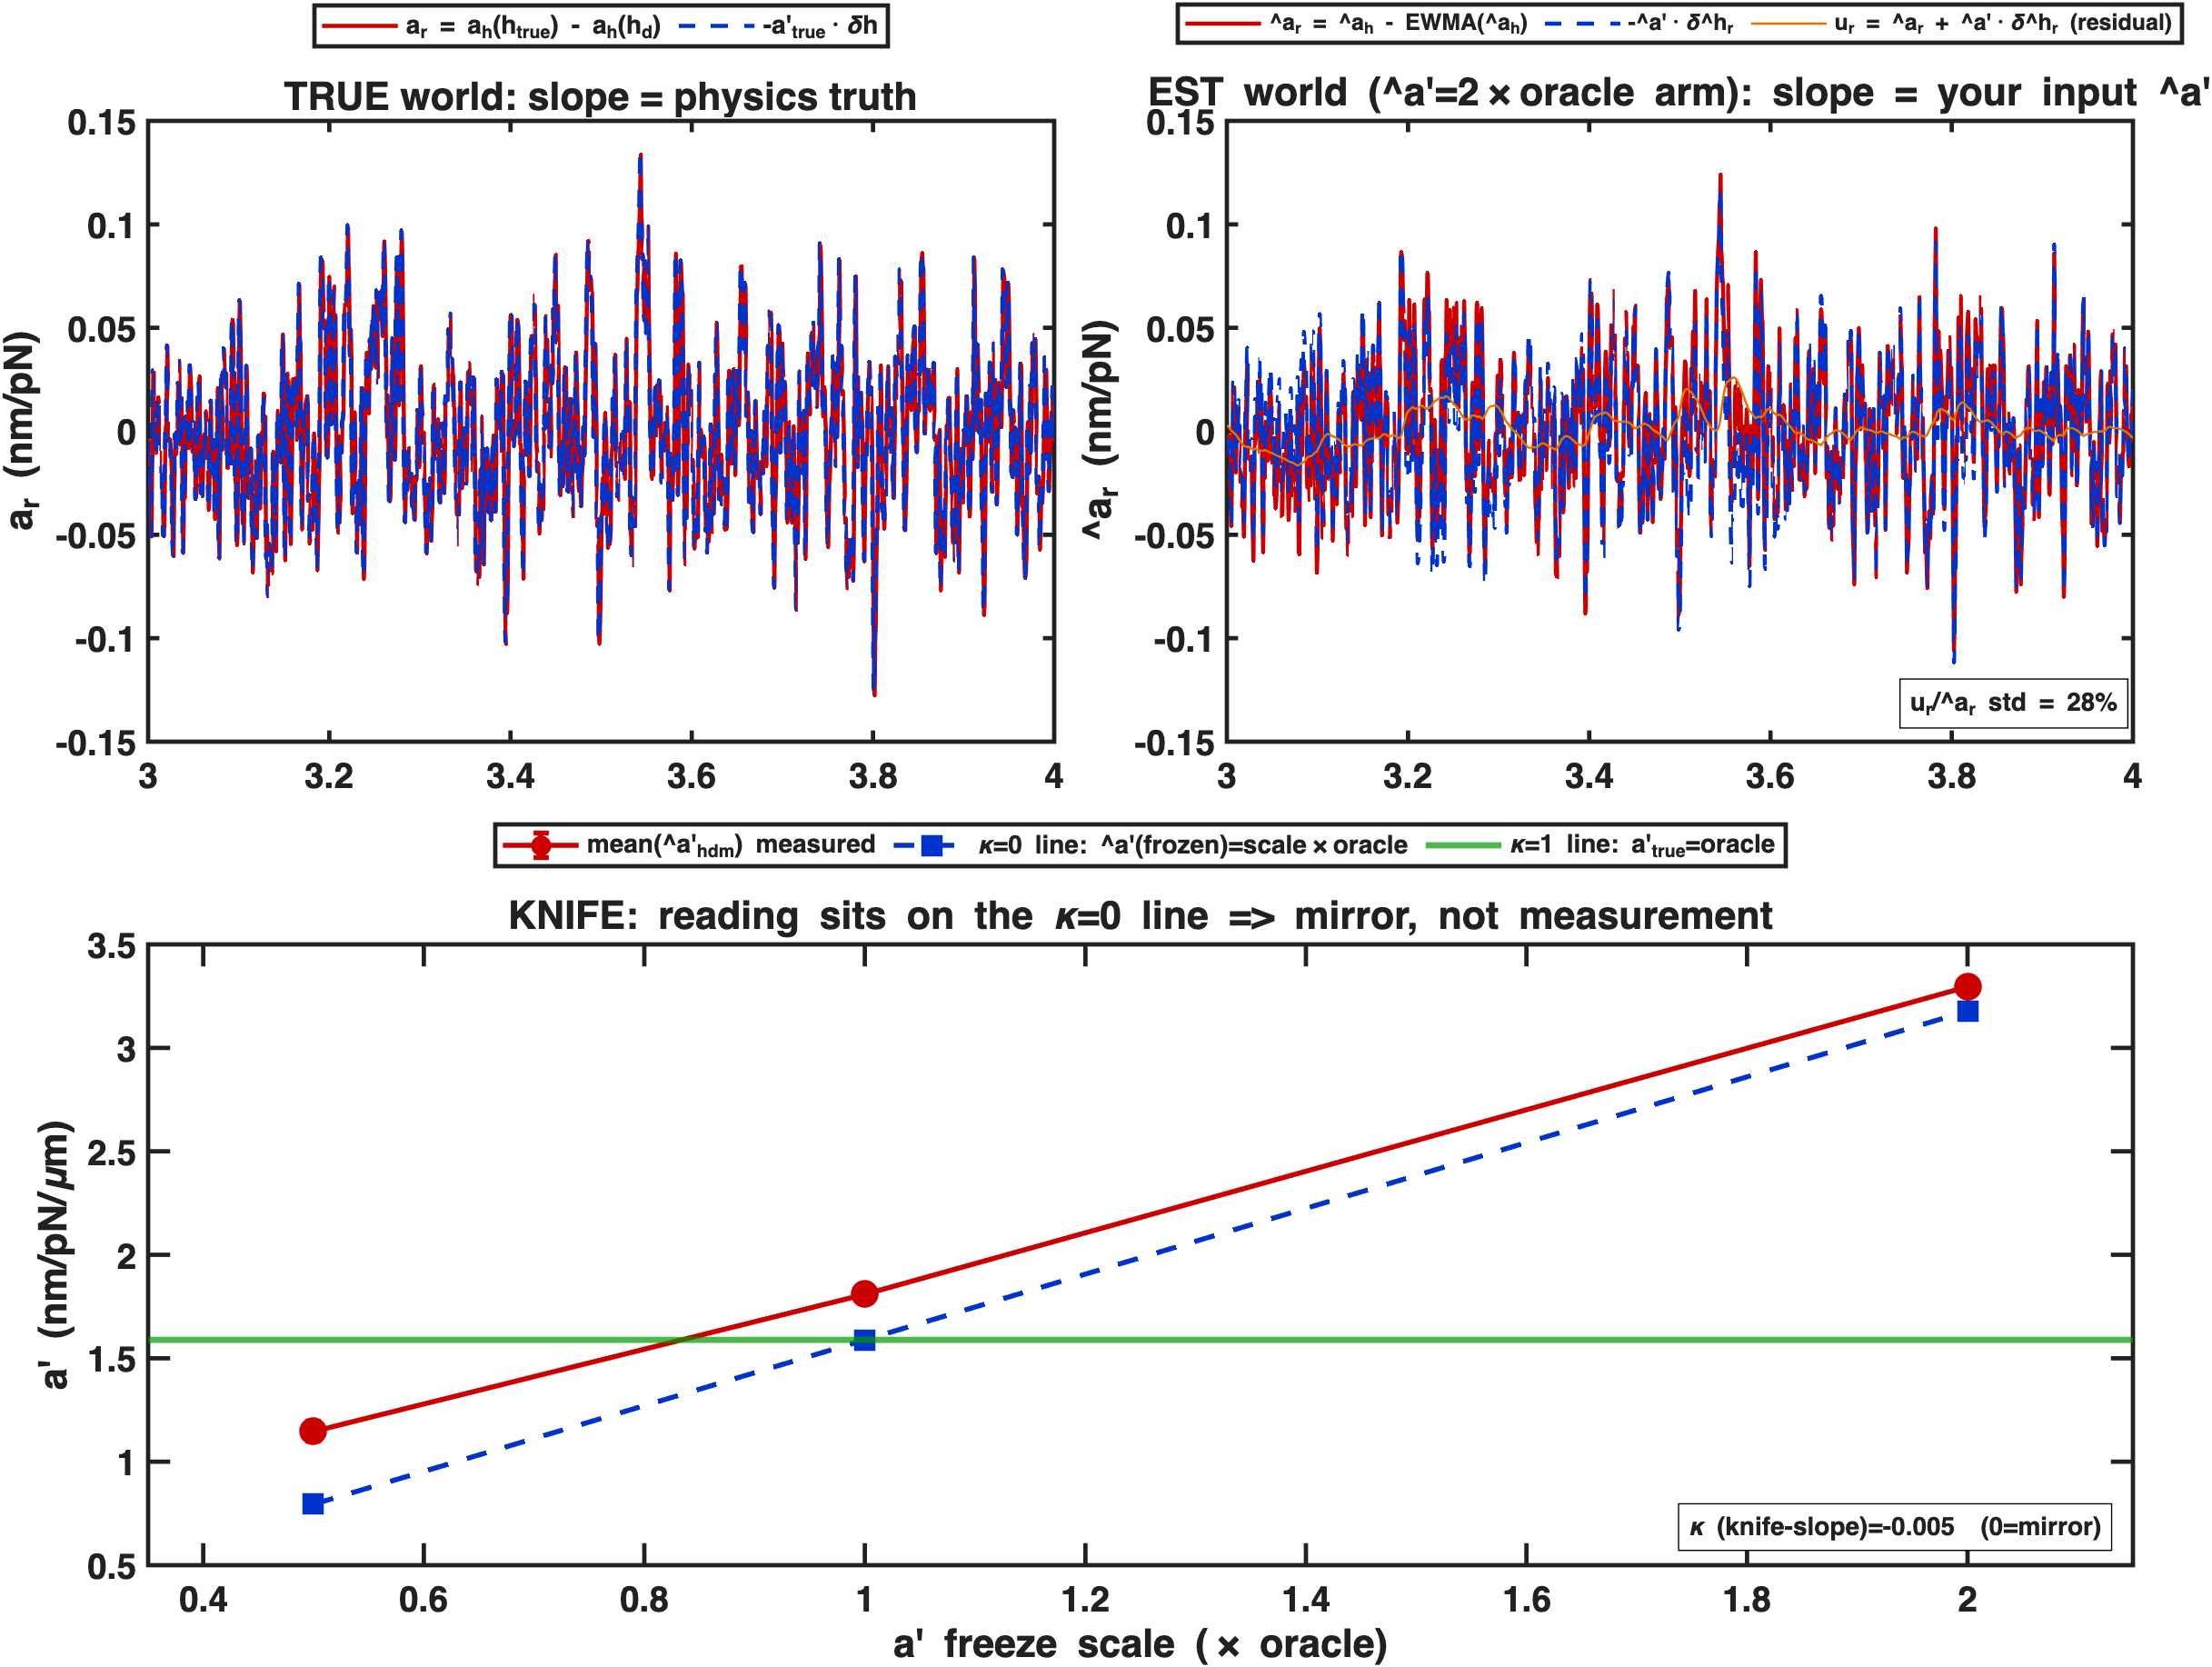
\includegraphics[width=0.98\textwidth]{figures/fig_mirror_hold_tier2.png}
\end{center}
\textit{Left (TRUE world): $a_r=a_h(h_{true})-a_h(h_d)$ overlays $-\ap\,\delta h$ --
slope is physics truth. Right (EST world, $\aph=2\times$oracle arm): $\hat a_r$
overlays $-\aph\,\delta\hat h_r$ (residual $u_r$ in orange) -- slope is your input
$\aph$, not truth. Bottom (KNIFE): the reading (red) sits on the $\kappa=0$ line
(frozen $\aph$), off the $\kappa=1$ line (oracle truth); $\kappa=-0.005$.}

\end{document}
